%!TEX root = ../thesis.tex
\chapter{Proposed Design} % (fold)
\label{ch:design}
This section describes the different choices in the interface for a digital newspaper and how the application can provide the user with an personal editorial mix.

Before it is possible express the editorial mix problem formally the interface of the application must be described, because the constraints will have to make some assumptions about the application structure. The two following sections will describe the layout and typography and the interaction with the application, respectively.

\section{Layout and Typography}% (Interface Design)
After the definition of the initial requirements was done the first prototype was developed. Its main features followed the requirements on turning pages, choosing an article, read it and returning to the overview of articles, see Figure~\ref{fig:prototype-iteration1}. And after a small preliminary survey it became clear, that a column-based layout showing full articles would be more attractive, and would provide a better opportunity to explore the editorial mix. With a column-based layout the digital newspaper would have more resemblance to conventional newspapers and therefore it was possible to apply some of the same principles of the editorial mix.
\begin{figure}%
%\centering%
\makebox[\textwidth][r]{% %%% as above; this time, the
%%% figures flushes from the left
\subfloat[Initial prototype layout with adjustable ratios between articles and a paged interface of each section.\label{fig:prototype-iteration1}]%
	{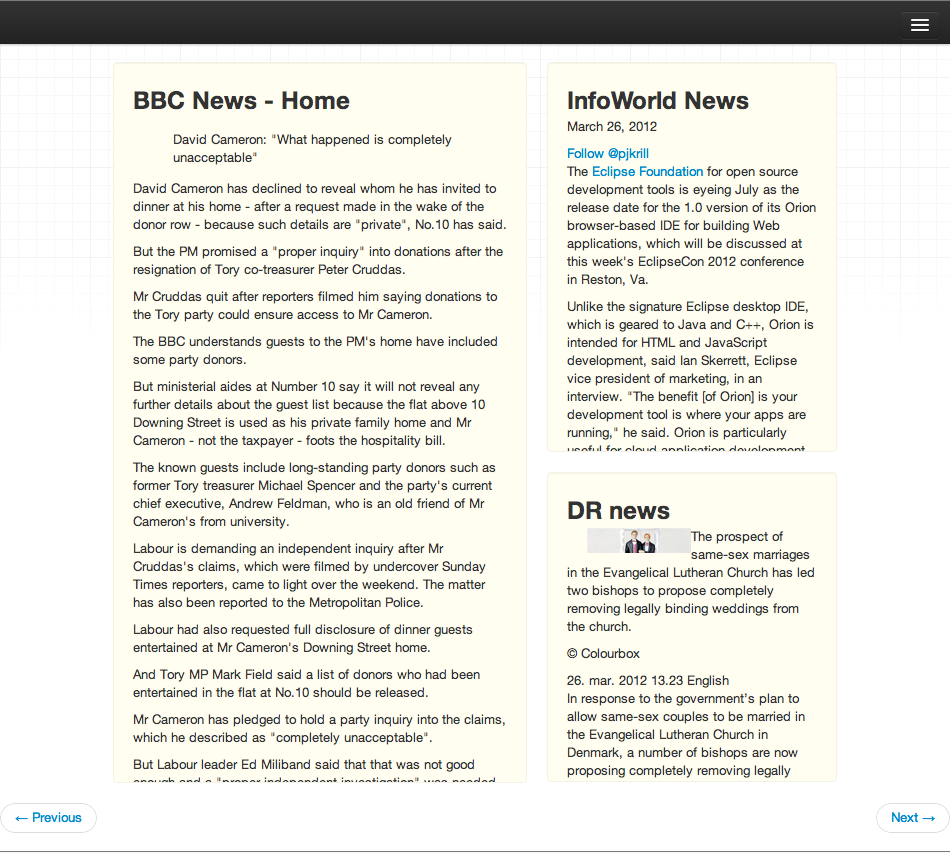
\includegraphics[width=.38\largefigure]{img/prototype-iteration1}}%
	\qquad%
\subfloat[Second iteration of the prototype with an ``endless'' layout. Sections are placed beneath each other.\label{fig:prototype-iteration2}]%
	{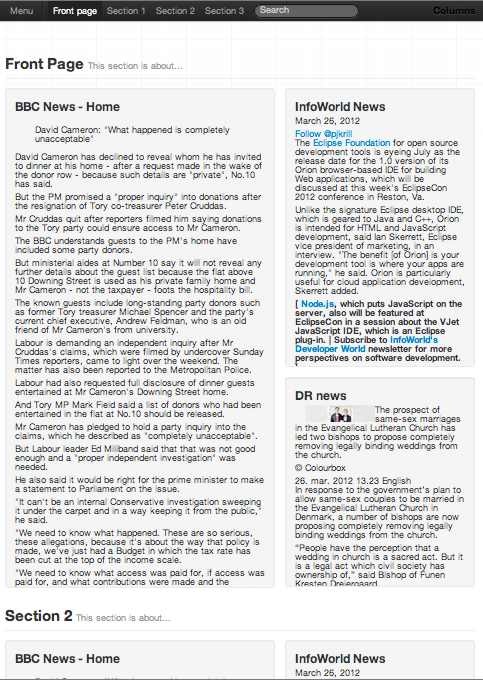
\includegraphics[width=.38\largefigure]{img/prototype-iteration2}}%
}
\\
\makebox[\textwidth][r]{% %%% as above; this time, the
\subfloat[Third iteration of the prototype with a column-based and ``endless'' layout. Sections are placed beneath each other.\label{fig:prototype-iteration3-1}]%
	{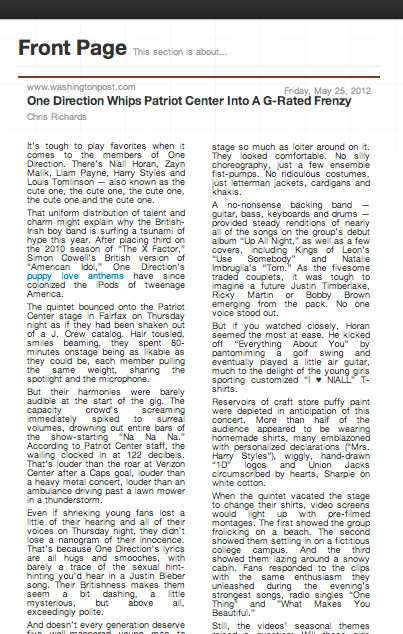
\includegraphics[width=.38\largefigure]{img/prototype-iteration3-1}}%
	\qquad%
\subfloat[Third iteration of the prototype with a column-based and ``endless'' layout. Sections are placed beneath each other.\label{fig:prototype-iteration3-2}]%
	{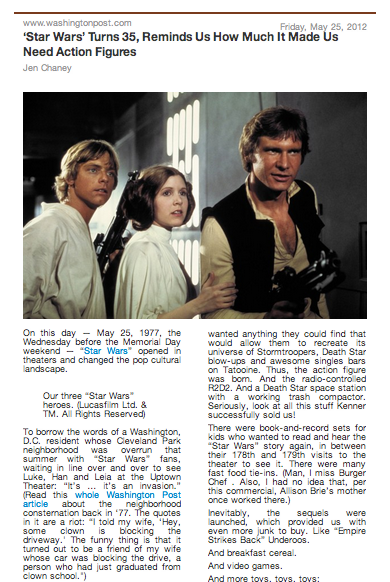
\includegraphics[width=.38\largefigure]{img/prototype-iteration3-2}}%
}
\caption{The figure shows three iterations of the prototype layout.}%
\label{fig:prototype-iterations}%
\end{figure}

Figure~\ref{fig:prototype-iterations} shows three iterations of the prototype design, which were based on the derived requirements. The third iteration of the prototype was used as the foundation for user tests. The prototype consisted of the basic navigation between topic categories, i.e.\ sections, and articles. Navigational choices was made in order to present the general idea of the framework, but where more crucial choices on its uses have not been made jet. This was also to encourage the test subjects to talk about what uses they would have of the presented framework. However, they were also asked about the navigational structure and indeed some changes had to be done. A specification of the test can be found in Table~\ref{tab:test-description}.
\begin{table}[h!tp]
	\myfloatalign
	\marginnote{
		\begin{minipage}{\marginparwidth}
		\vspace{-100pt}
		\caption{Test Specification}
		\label{tab:test-description}
		\end{minipage}
	}
	\makebox[\textwidth][l]{
		\begin{tabularx}{.8\largefigure}{p{.15\largefigure}|p{.6\largefigure}}
		\toprule
			\textbf{Test subjects} & The test was conducted on a total of 7 test subjects of ages between 21-29, and of different sex and occupation.\\
		\midrule
			\textbf{Participants} & Each test was done with 1 test conductor and 1 test subject.\\
		\midrule
			\textbf{Materials} & An iPad with the application running and a computer to write notes on the test subject's statements and propositions.\\
		\midrule
			\textbf{Description} & The test subject was presented with the prototype layout seen in Figure~\ref{fig:prototype-iteration3-1} and~\ref{fig:prototype-iteration3-2}. The test was conducted as an informal qualitative talk with a basis in the test subject's interests in such a product. Transcripts from each test can be found at \url{http://lestrade.imm.dtu.dk/~s062596/data/test-transcripts.zip} and a summery of the results in section~\vref{sec:test_results}.\\
		\bottomrule
		\end{tabularx}
	}
\end{table}

The main points from the user test was that the newspaper should provide an overview of its contents, that it should be easy to navigate relevant new and archived articles, that the users wanted to provide relevance feedback on articles and indication of the relevance of the article. Moreover, the newspaper should provide a good balance between imagery and textual content, that white space in between articles is not a problem and that an article should be read screen by screen, even if it means dividing text into a new set of columns. It was pointed out that some problems may arise if there is not room enough in the top menu, e.g.\ when in portrait mode and, as the test subjects specifically requested, this could be solved by introducing a carousel-like arrow buttons to scroll the tabs, or even just using touch interactions. Moreover, the user should be able to read the newspaper screen by screen, meaning that trailing text should be put into a new set of columns whenever it exceeds the screen, see Figure~\ref{fig:reading1} and \ref{fig:reading2}.
\begin{sidefigure}%
	\vspace{-220pt}
	\myfloatalign%
	%\hspace{-17.8pt}
	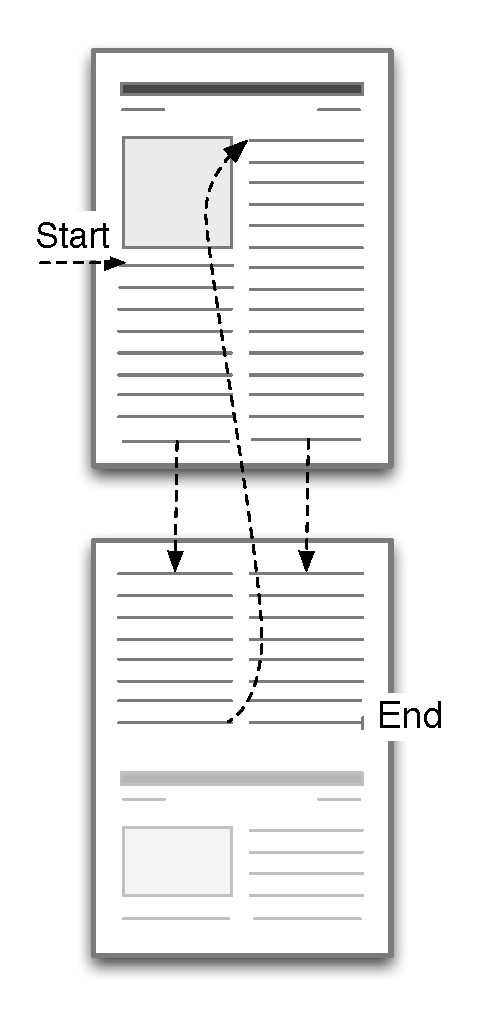
\includegraphics[width=\marginparwidth]{img/reading1} 
	\caption{Reading pattern where the user has to scroll in order to see the full length of the column.}%
	\label{fig:reading1}%
\end{sidefigure}

One user in particular expressed that the application had solved the problems that \url{http://nyhederne.tv2.dk/}\sidenote[1]{The website of a Danish news channel.} has and given the additional features it would provide a readable layout, easy navigation and a good overview of its content. No user expressed the need for any general news as presumed in the scenarios, only personalised news was of preference to the test subjects. They argued that if they wanted news of some kind, they would just create a section for it. Even so \cite{fulltext.pdf} argues that common sense dictates some ``breaking'' articles to be universally interesting and that the problem of some user may not receive them\sidenote[1]{This is also known as the black sheep problem.} could be solved be collaborate filtering. Collaborate filtering is a good way apply wisdom of the crowd to the application, which might make it stronger as the number users grows. Finally according to the user tests, it should be chosen from which period the articles should come from, as opposed to what was extracted from the scenarios and respondents from \cite{FULLTEXT01.pdf} which suggests that the paper should be continuously updated.

\begin{sidefigure}%
	\myfloatalign%
	%\hspace{-17.8pt}
	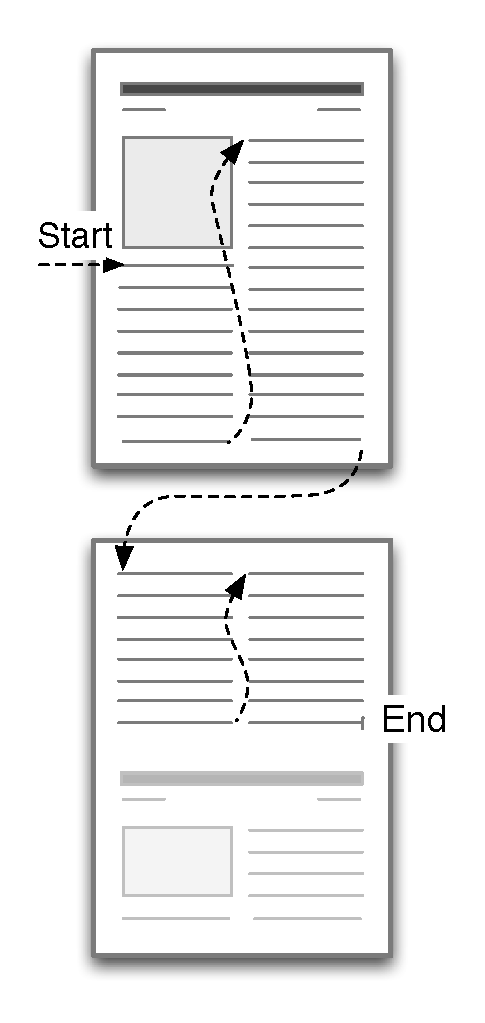
\includegraphics[width=\marginparwidth]{img/reading2} 
	\caption{Reading pattern where the user can finish reading a whole page before scrolling to read the next.}%
	\label{fig:reading2}%
\end{sidefigure}

Based on the user feedback a new design was developed. It is seen in Figure~\ref{fig:mockups}.
\begin{figure}%
\myfloatalign
\makebox[\textwidth][r]{
	\subfloat%
			{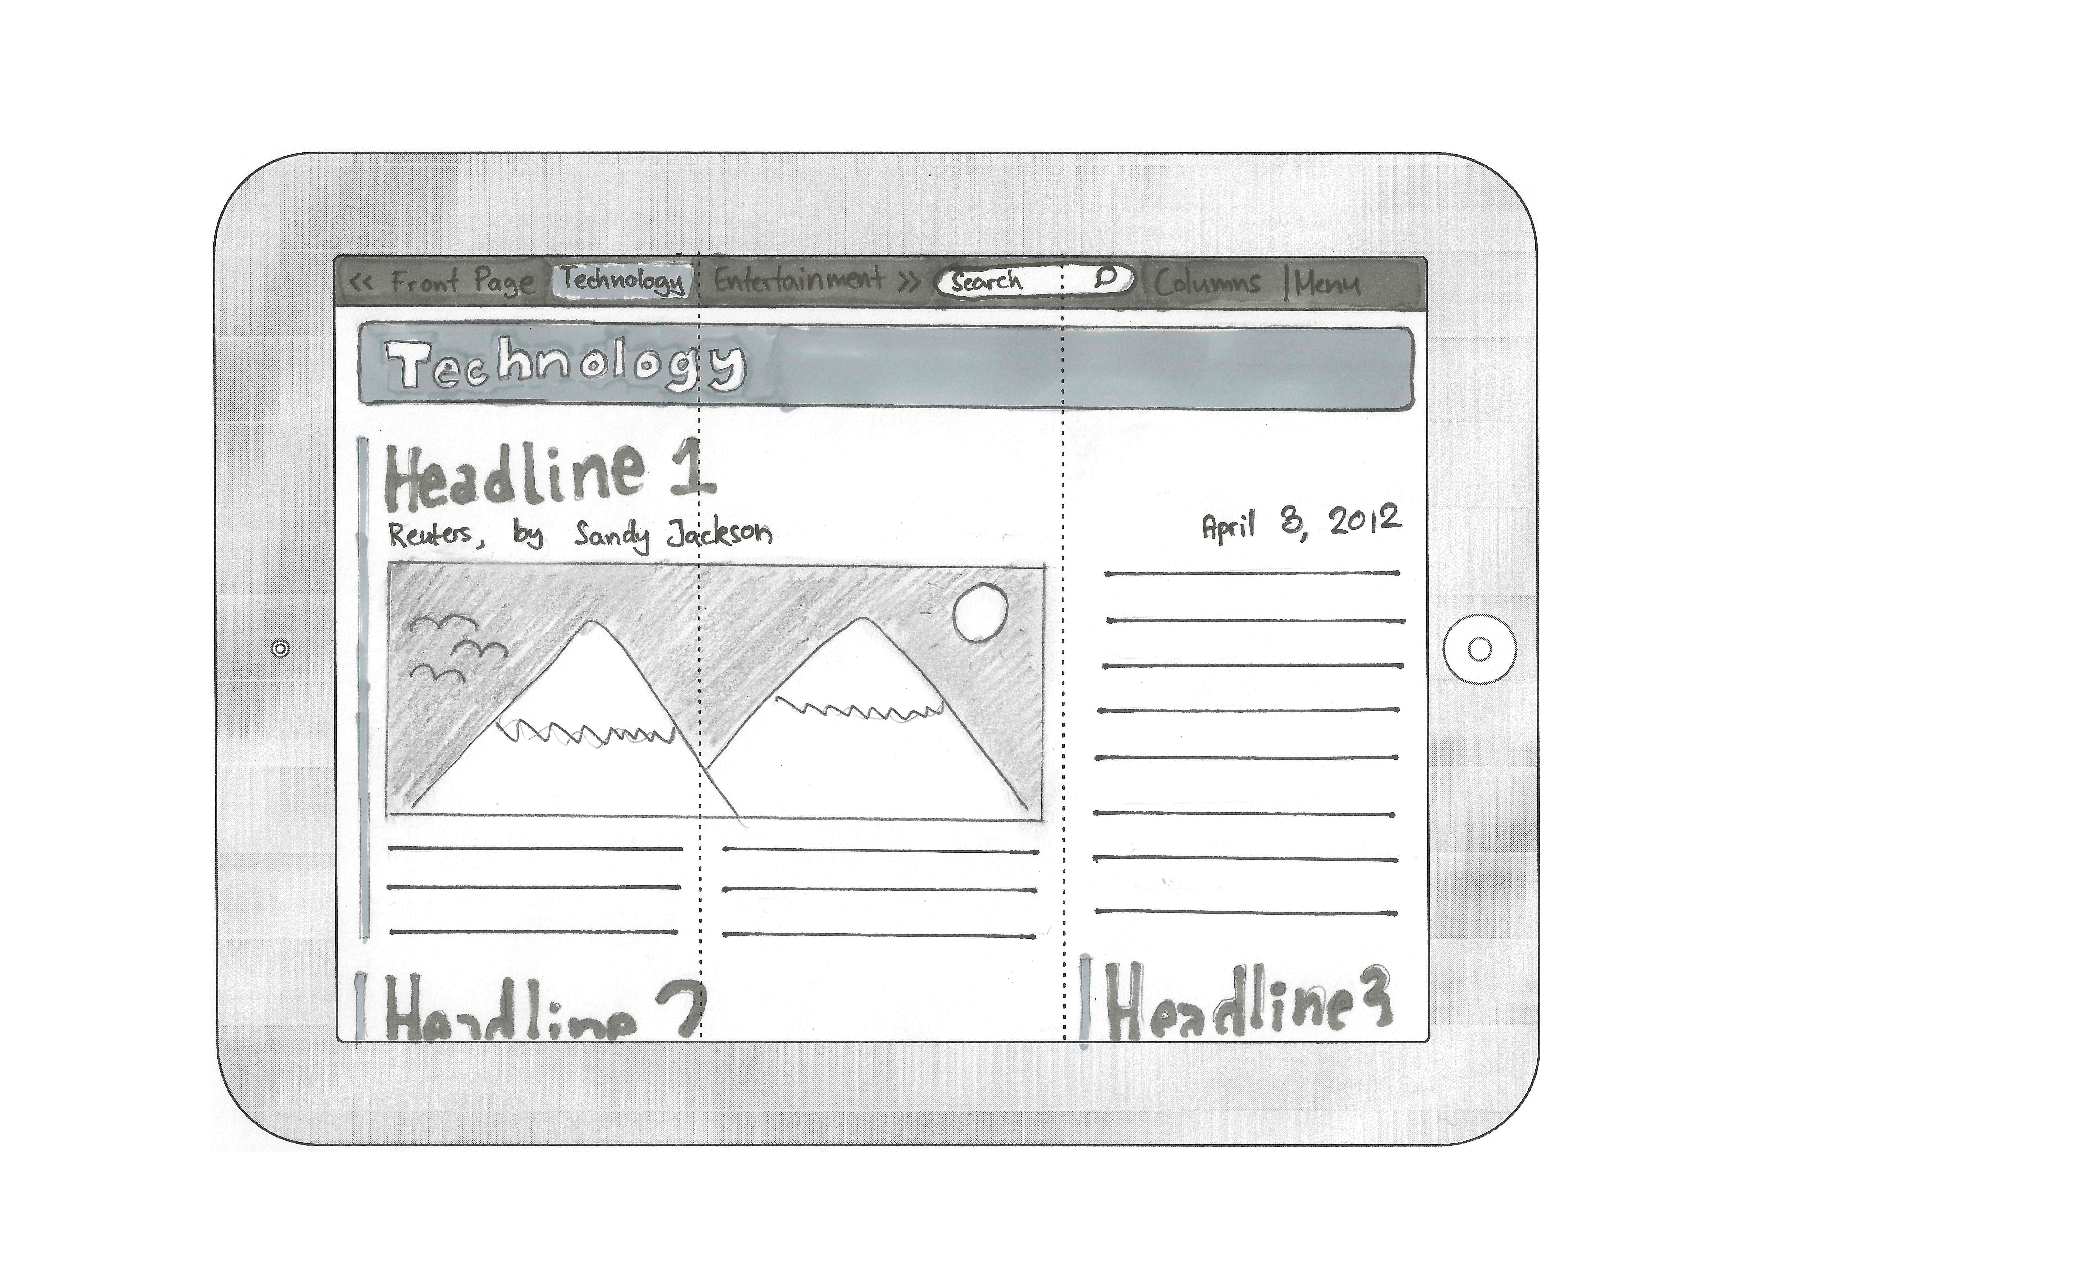
\includegraphics[width=.43\largefigure]{img/mockup-landscape}}
		\qquad
	\subfloat%
		{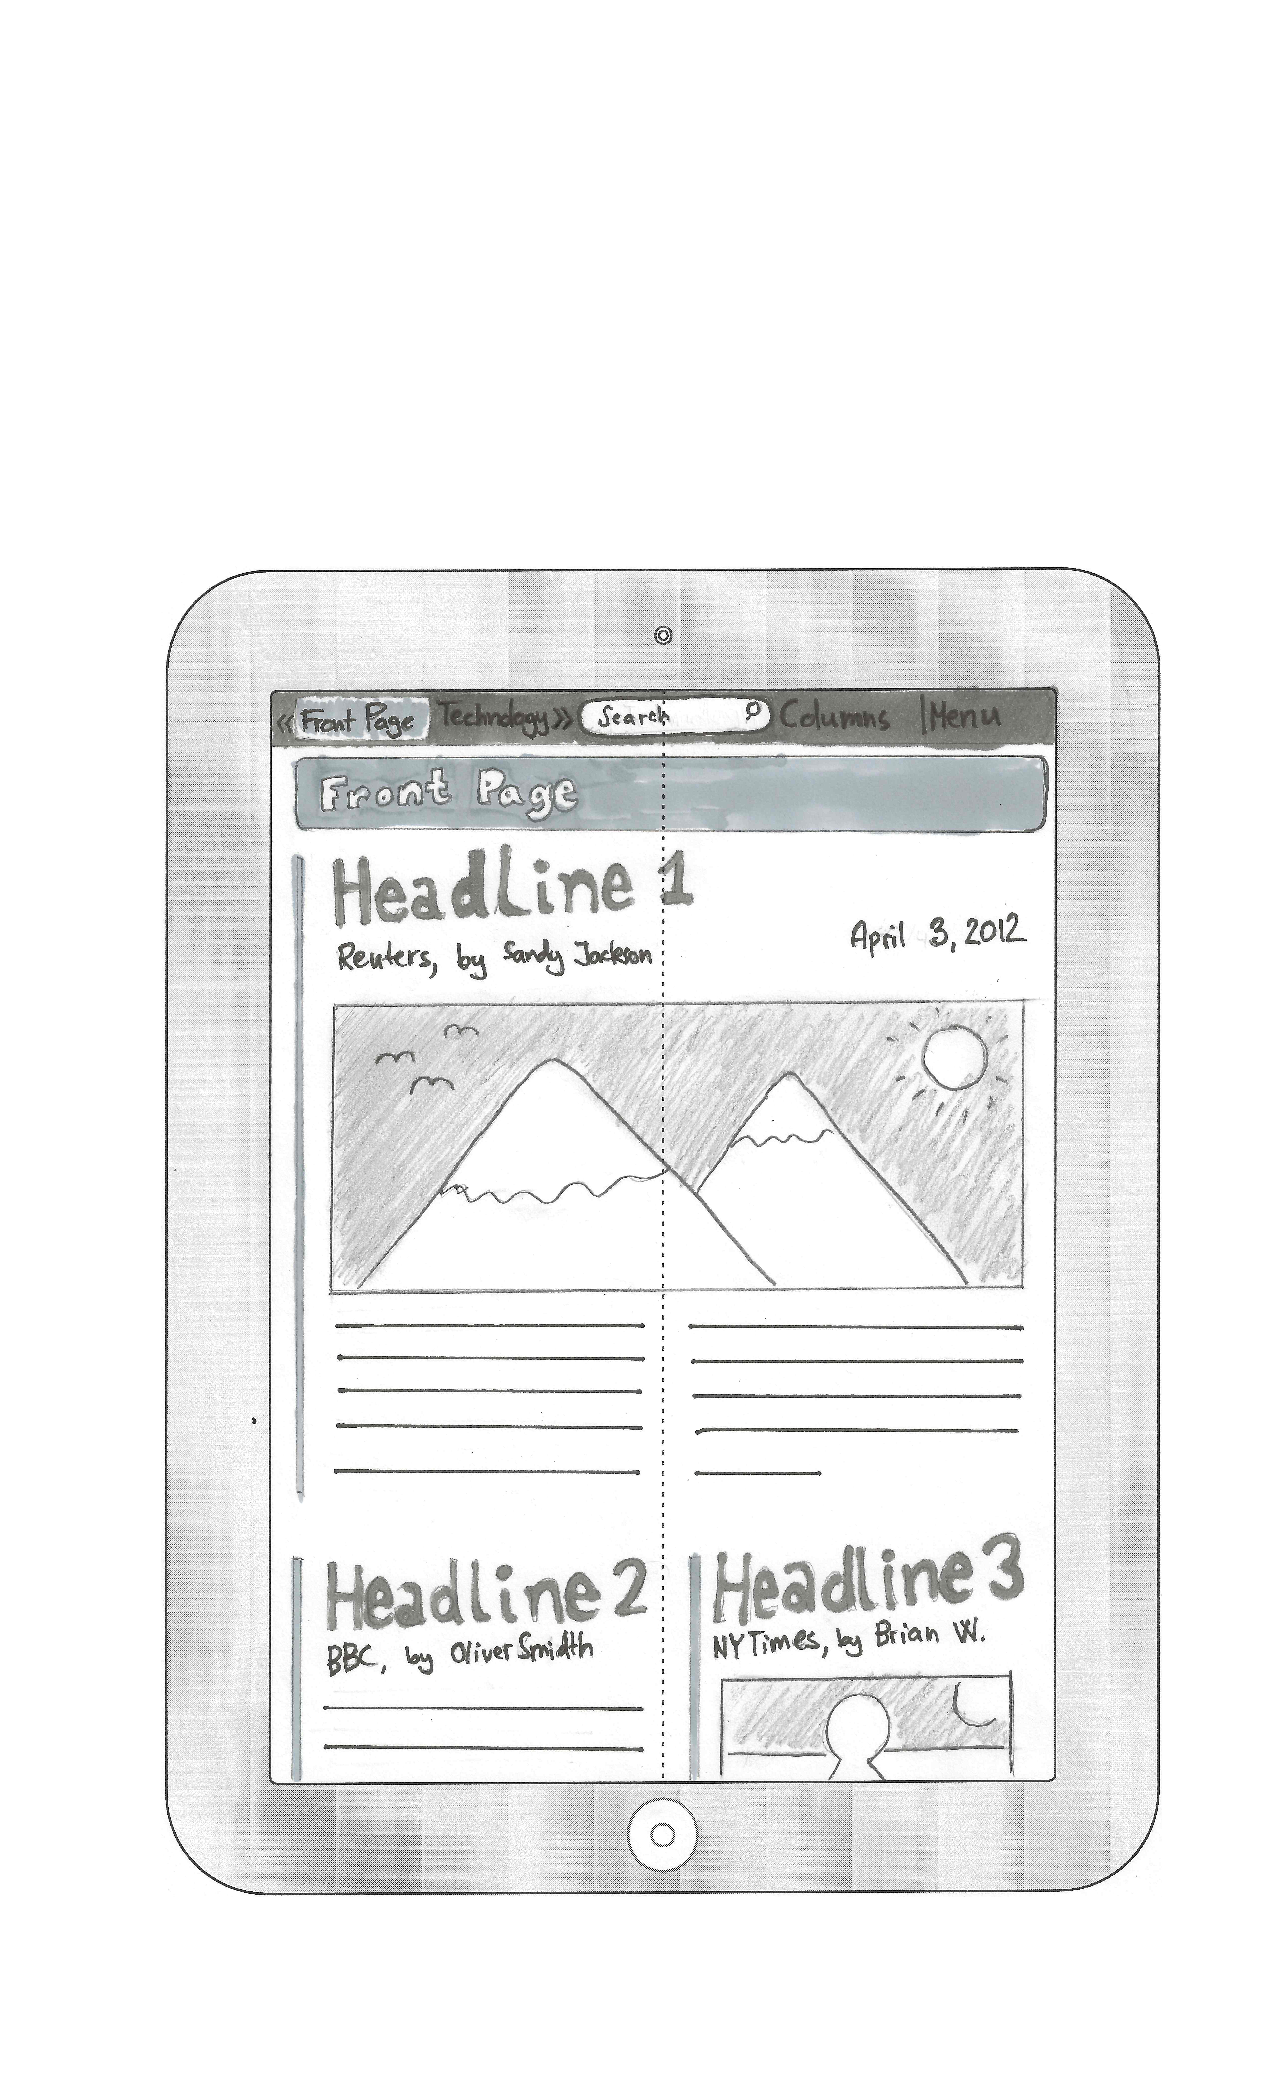
\includegraphics[width=.33\largefigure]{img/mockup-portrait}}
}
\marginnote{
	\begin{minipage}{\marginparwidth}
		%\vspace{-100pt}
		\caption{\\The figure shows mockups of the layout in landscape and portrait mode, respectively.}%
		\label{fig:mockups}%
	\end{minipage}
	}
\end{figure}

The top menu from the prototypes is kept, but arrows are added to solve the problem of overflow if the items gets too numerous. That the menu presents the items along side each other supports the fact that sections visually lie beside each other in the navigational space, i.e.\ the user can flick (see Figure~\ref{fig:flick}) the section and an animated transition slides the section out and the next in.
\begin{sidefigure}[h!tp]
	\myfloatalign
	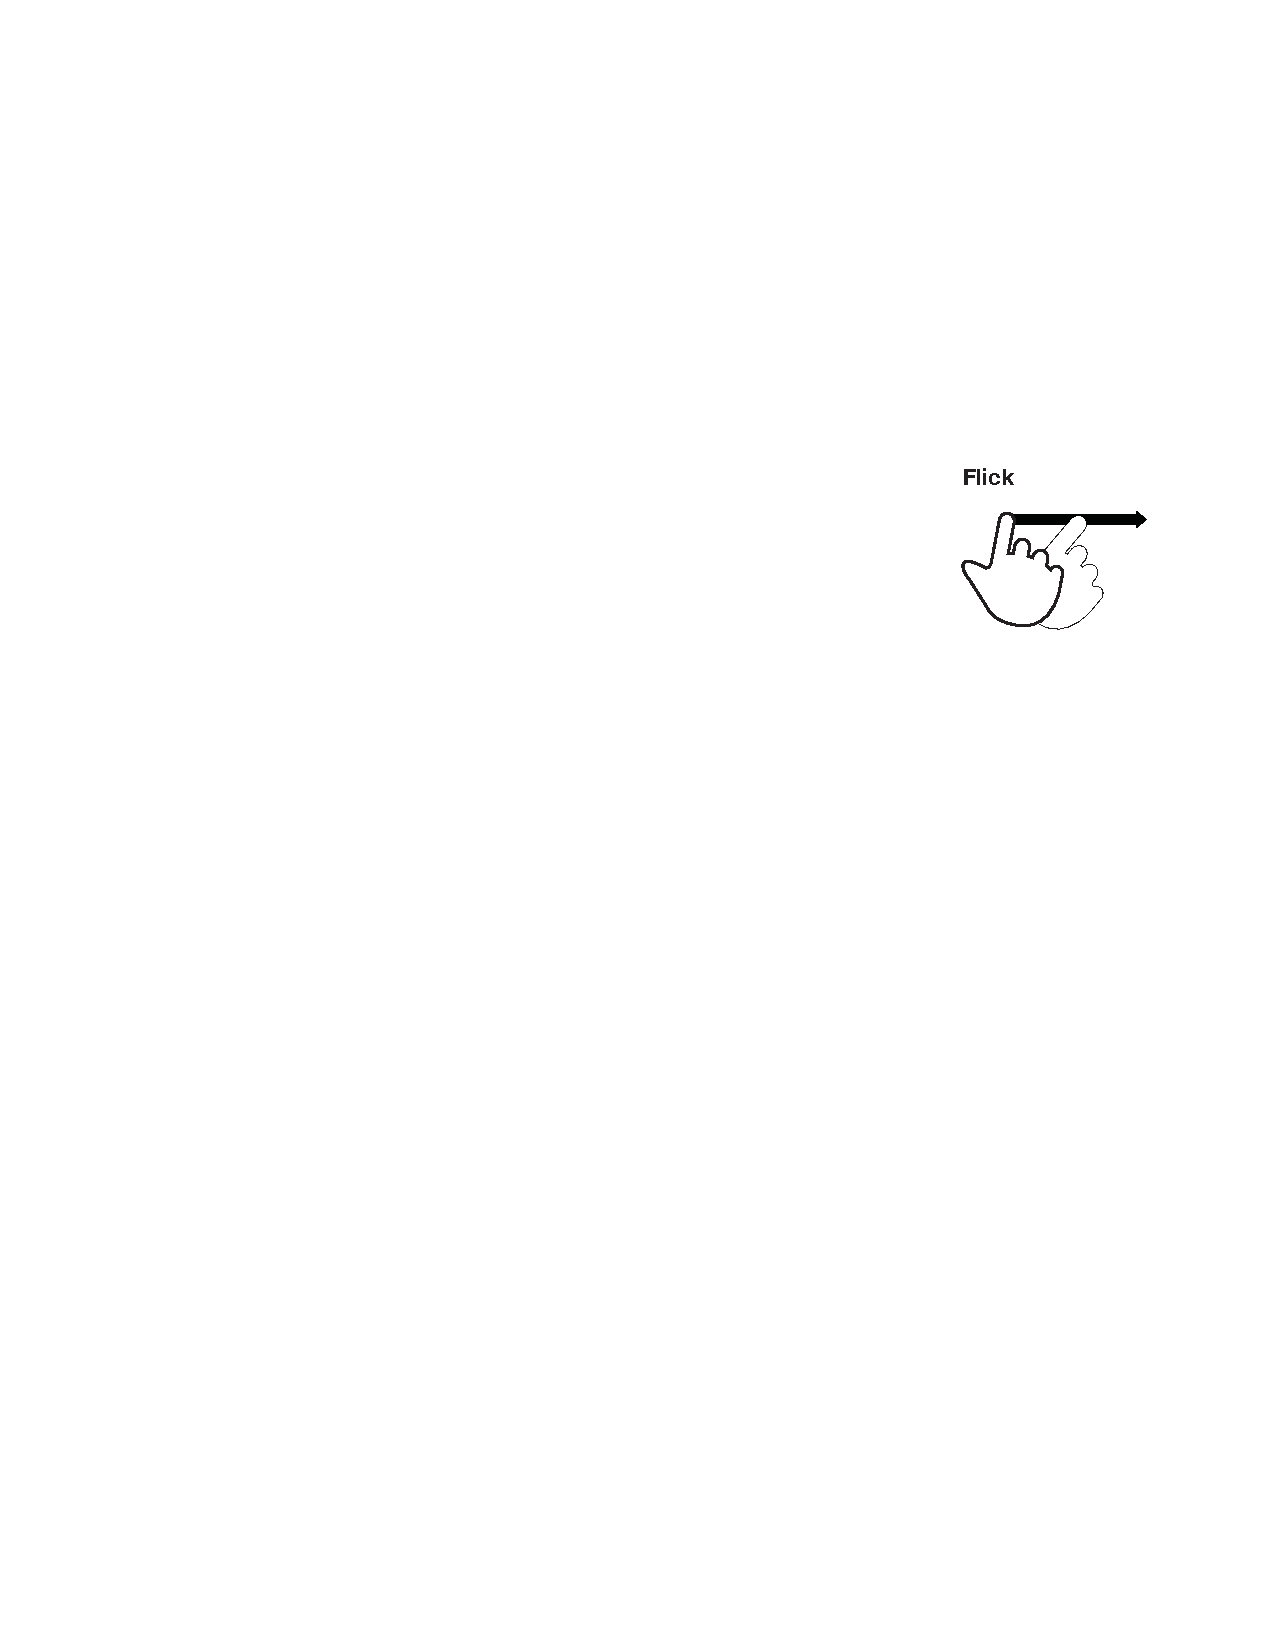
\includegraphics[width=\marginparwidth]{img/flick}
	\caption{Touch gesture: Quickly brush surface with fingertip.}
	\label{fig:flick}
\end{sidefigure}

The top menu bar is given a dark colour to provide some visual contrast from content to functionality. In the new layout articles are shown in full and images are maximised. Rules of readability determines, as opposed to that on print, that small point size text work better with a sans-serif font \cite{Tidwell}. The neutral Helvetica has therefore been chosen as the body text, whereas the article headlines are the most important thing on the page, and therefore are supplied with the largest typeface. To separate them further from the body text a serif font has been used. The section headers are assigned with a medium size, but wide, font because the user needs to navigate using this headline. However, the user already knows the name of the section (he has probably given it himself) and does therefore not necessarily need to read it - just recognise it. On this background the section headline is placed in a bar and supplied with the same light colour as the background. This makes them more neutral, but still easy to navigate using the bar. To relate the paratext with the section they are supplied with the same colour as the section bar. This should let the user associate the article with the topic of the section. Furthermore, a the line that was on top of the articles (see Figure~\ref{fig:prototype-iteration3-2}) is moved to be beside it. This is visually indicate when an article starts and ends. This will also aid to understand that the article continues if the article columns should be divided into screen sizes. Again the same colour as the section bar is used to set both the visual and contextual frame.

In the prototype the menu consisted of all the settings in a modal panel, but the test subjects wanted a division between visual tools, e.g.\ changing size of the font or colour scheme, and the content settings, i.e.\ the control of what each section should contain. The former is moved into a side menu with a button to access the latter, which kept in a modal panel. This way the handy visual tools are only one interaction away, whilst the more complex settings are hidden away with two interactions. And the overview of article headlines in the section could be done as in Sublime Text 2\sidenote[1]{Sublime Text 2 is a text editor for coding.}, see Figure~\ref{fig:sublime}
\begin{figure}[h!tp]
	\myfloatalign
	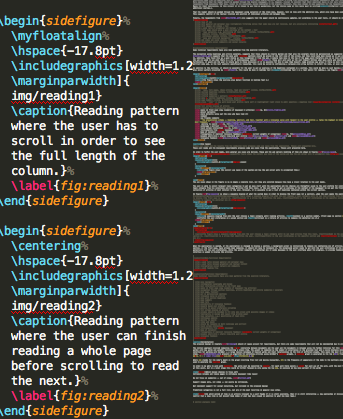
\includegraphics[width=.5\textwidth]{img/sublime}
	\marginnote{
		\begin{minipage}{\marginparwidth}
			\caption{The figure shows the overview plus detail function in Sublime Text 2.}
			\label{fig:sublime}
		\end{minipage}
	}
\end{figure}

This overview could be placed in the side menu and show a larger (and readable) scale of headlines and the user should be able to see the images further down in the newspaper.

\section{Interactions}% (Interface Design)
In Figure~\ref{fig:navigation} is the navigational of the application structure outlined. 
\begin{figure}[h!tp]
	\myfloatalign
		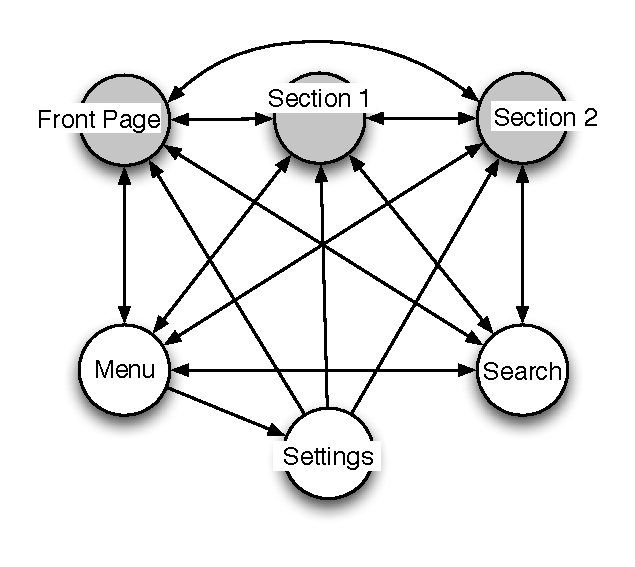
\includegraphics[width=.45\textwidth]{img/navigation}
	\marginnote{
		\begin{minipage}{\marginparwidth}
			\caption{The figure shows the navigational structure of the application.}
			\label{fig:navigation}
		\end{minipage}
	}
\end{figure}

The three sections are holds the contents of the newspaper, which can be extended with additional sections through the settings menu. The sections lay along side each other in the navigational space and it is possible to navigate to sections beside the current through the flick gesture, but through the top menu it is possible to go directly to any of the sections. Because the top menu is visible at all times except when in the settings menu, it is possible to go directly to any of the sections and do a search anywhere from the application, except of cause from the settings menu. This means that the application is very interconnected and since the settings menu is meant to be used rarely the extra navigational step does not matter. The settings menu should only be used the first time the user opens the application to adjust the basic settings and then afterwards only to correct if the application does not comply with the user preferences, or when the super user wants to adjust the settings. In a perfect world the user would never have to open the settings menu to adjust anything, only observe while the application learns the user interests and delivers what is expected.

When the user is at first presented with the application he should have as a direct path as possible leading to actually reading articles, which is of main user needs. He is presented with a form to make choices about the contents of the newspaper. The application provides the possibility for choosing whether the front page should be visible or not. This functionality is given to the user that would rather just have his sections and no front page. After this the user can choose the topic for the first section from a list of predefined topics. If the topic he is looking for is not in the list he can choose to fill out some keywords to cover his interests. After this he can provide it with a name for the section and choose to add another section or save his user profile. It is also possible for him to choose how many articles he would like in each section, including the front page. Figure~\vref{fig:mockup-form} shows a mockup of the settings menu.
\begin{figure}[h!tp]
	\myfloatalign
		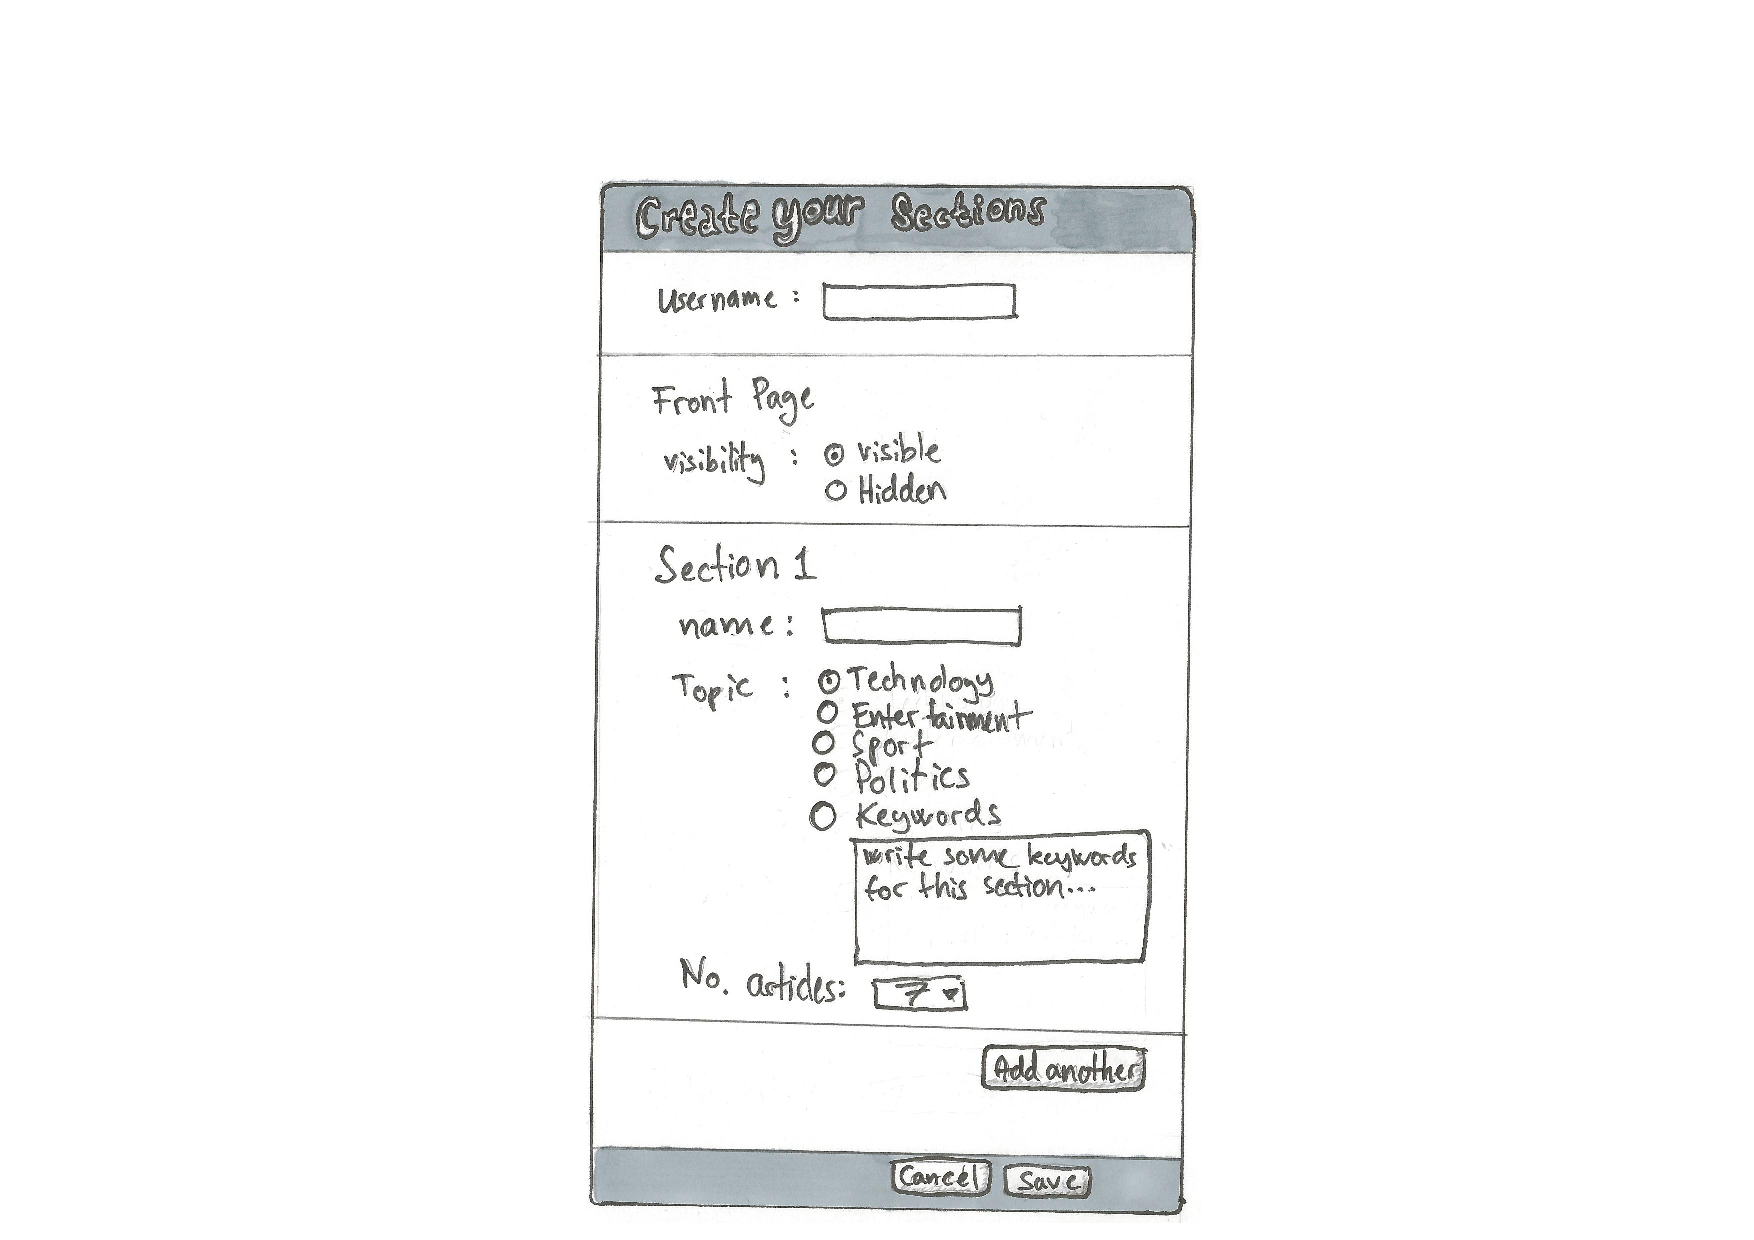
\includegraphics[width=.45\textwidth]{img/mockup-form}
	\marginnote{
		\begin{minipage}{\marginparwidth}
			\caption{The figure shows mockup of the form that constitutes the settings menu.}
			\label{fig:mockup-form}
		\end{minipage}
	}
\end{figure}

To be able to solve the editorial mix problem using CP it must be expressed as a COP and the presented constraints must be translated to logical constraints. This is done in the following section.

\section{Problem Representation}
The division of rules between the front page and the section can be kept in the problem representation, which will, as we will see later, be the source for the possibility of incorporating lazy loading of each section. This section will therefore present a general problem specification for a section, which can be used in every section and on the front page, with varying constraints. Also, the front page will through this section and the following be referred to as a section, and specifically as section $0$.

The set of values, $\mathcal{V}$, from equation~\vref{eq:problem_spec} in the problem is represented by a library of currently available articles and the set of variables, $\mathcal{X}$, is represented by the available positions in the section. Each variable can then be assigned a value in the form of a specific article and when a complete assignment satisfies all constraints, a solution has been found. An article consists of a set of attributes, e.g.\ a date, the number of words in the article and a number indicating a relevance. Constraints are defined on variables and through them bound to their specific places in the section.

In the following the constraints presented in section~\vref{sec:analysis_mix} will be formulated as logical constraints divided into general constraints for all sections and specific constraints for the front page and other sections, respectively. Constraints defined on variables with letters, e.g.\ $x_a$ and $x_b$, means that the constraint is defined for every combination of variables from the problem. Hard constraints returns whether it is satisfied and preference constraints returns a violation, where $0$ means not violated.

\paragraph{General Unary Constraints}
\begin{align}
	\begin{Bmatrix}
		\texttt{time-frame}(x_a) &\rightarrow& x_a.date >= today-7,\\
		\texttt{featured-space}(x_a) &\rightarrow& x_a.featured = \texttt{false}\ \vee\\
			&&x_a.columns = 2\ \vee\\
			&&x_a.columns = 3,\\
		\texttt{nonfeatured-space}(x_a) &\rightarrow& x_a.featured = \texttt{true}\ \vee\\
			&&x_a.columns = 1\ \vee\\
			&&x_a.columns = 2,\\
		\texttt{featured-image}(x_a) &\rightarrow& x_a.featured = \texttt{false}\ \vee\\
			&&x_a.has\_image = \texttt{false}
	\end{Bmatrix}
\end{align}
%\texttt{\textbf{if}}(
%)\\
%&&\texttt{ \textbf{return} } 0 \texttt{ \textbf{else return} } 1

Where $n$ is the number of positions and therefore variables, in the section and $today$ is variable that holds the current date. The \texttt{time-frame} constraint is set to include articles from a week ago, but can of cause be adjusted. As the layout is defined in 2 and 3 columns the \texttt{featured-space} constraint is satisfied only when the article fills out 2 or three 3 columns. Likewise with the \texttt{nonfeatured-space} which is only satisfied with articles that fills 1 or 2 columns. \texttt{featured-image} is a constraint, to control that a featured article should have an image. These three constraints could be used as they are, but could also function as assignments along with a calculation of the relevance to base the rest of the constriants on, i.e.\ to determine that a featured article is an article with many words, has an image and has a lot of relevance; otherwise it is not.

\paragraph{General Binary Constraints}
%\begin{minipage}{.8\largefigure}
\begin{align}
\hspace{-60pt}
	\begin{Bmatrix}
		\texttt{featured-adj}(x_a, x_b) &\rightarrow& \texttt{not adjacent}(x_a,x_b)\ \vee\\
			&&(x_a.featured = \texttt{false}\ \wedge\\
			&&x_b.featured = \texttt{false})\ \vee\\
			&&x_a.featured = \texttt{true}\ \wedge\\
			&&x_b.featured = \texttt{true},\\
		\texttt{featured-pos}(x_a, x_b) &\rightarrow& \texttt{not adjacent}(x_a,x_b)\ \vee\\
			&&(x_a.featured = \texttt{false}\ \wedge\\
			&&x_b.featured = \texttt{false})\ \vee\\
			&&(x_a.featured = \texttt{true}\ \wedge\\
			&&x_a.position > x_b.position)\ \vee\\
			&&(x_b.featured = \texttt{true}\ \wedge\\
			&&x_b.position > x_a.position),\\
		\texttt{adj-subj}(x_a, x_b) &\rightarrow& \texttt{\textbf{if}}(\texttt{not adjacent}(x_a,x_b))\\
			&&\texttt{\textbf{return} max}(0,\\
			&&64 \cdot \texttt{similarity}(x_a,x_b)^2\\
			&& - 64 \cdot \texttt{similarity}(x_a,x_b)\\
			&& + 15.36)\\
			&&\texttt{\textbf{else return }}0
	\end{Bmatrix}
\end{align}
%\end{minipage}
Where $\texttt{max(number,\ number)}$ is a function that returns the maximum of the given numbers and $\texttt{similarity}(variable,\ variable)$ is a function that returns the mutual similarity between the values of two given variables. These general binary constraints control most of the editorial mix, because they express that to featured articles should not be placed adjacent to each other, that featured articles should be placed higher than its adjacent non-featured articles and that adjacent articles should have the same subject. The latter is a preference constraint because some uncertainty is introduced when controlling that two articles should have the same subject. That articles have the same subject can approximately be determined by how similar they are to each other, i.e.\ if the articles are much too similar they could be articles on the same story, and if they differ too much, they may be on a different subject. However, in between should roughly determine that the articles are on the same or a similar subject, which is what is needed. In the \texttt{adj-subj} constraint this is done by the returning a violence based on the parabolic function seen in Figure~\ref{fig:curve}.
\begin{figure}%
\myfloatalign
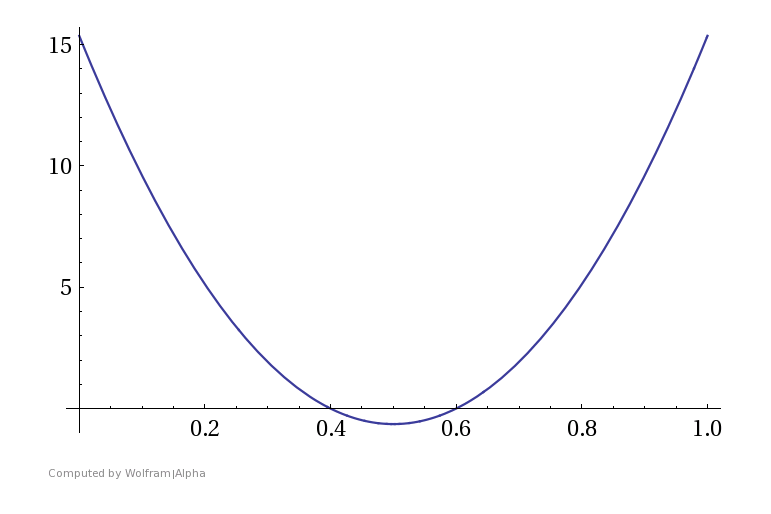
\includegraphics[width=.45\textwidth]{img/curve}
\marginnote{
	\begin{minipage}{\marginparwidth}
		\caption{Plot of $64 x^2 - 64 x +15.36$.}%
		\label{fig:curve}%
	\end{minipage}
	}
\end{figure}

If the similarity of the two articles are below $0.6$ or above $0.8$, than its distance to this point will determine its violence by the parabolic function. These numbers are of cause adjustable and will vary according to the selected similarity function, but are given to show a more expressive example.
%(-1.4a+sqrt((-1.4a)^2-4a(-0.1+0.49a)))/(2a)=0.8
%(-14/225+sqrt((-14/225)^2-4*2/45*137/1125))/(4/45)
\paragraph{General Global Constraints}
\begin{align}
	\begin{Bmatrix}
		\texttt{all-diff}(x_1,\ldots,x_n) &\rightarrow& \bigwedge\limits_{i=1,\dots,n}\bigwedge\limits_{j=1,\dots,n}\ \texttt{similarity}(x_i,x_j) < 0.9
	\end{Bmatrix}
\end{align}

The final of the general function determines that every article must be different. In the constraint this is expressed by checking if the similarity between the articles is too high, it could also be done by just checking the id, but this might introduce more of the same story, but from different content providers.
%\begin{itemize}\itemdist
%%\subsubection{Unary}
%	\item An articles should be within a given time frame
%	\item A featured articles should be allowed to take up more space
%	\item A featured articles should be accompanied by an image
%	\item A non-featured article should take up less space
%%\subsubection{Binary}
%	\item A featured article should be adjacent to non-featured articles
%	\item A featured should have a higher position than its adjacent non-featured articles
%\item Articles should be grouped into subjects
%%\subsubection{Global}
%	\item All articles should be different
%\end{itemize}

\paragraph{Front Page Constraints}
\begin{align}
	\begin{Bmatrix}
		\texttt{main-stories}(x_a) &\rightarrow& \bigvee\limits_{i=1,\dots,g}\ \texttt{relevance}(x_a,i) >= 0.75,\\
		\texttt{nonfeatured-image}(x_a) &\rightarrow& \texttt{\textbf{if}}(x_a.has\_image) \texttt{\textbf{ return }}0\\
		&&\texttt{\textbf{else return }}1
	\end{Bmatrix}
\end{align}

Where $g$ is number of sections and $\texttt{relevance}(variable,\ section\ number)$ returns the relevance of the given variable in the given section number. The former constraint expresses the need for only articles of high relevance on the front page and the latter that nonfeatured articles preferably also should have images on the front page.
%\begin{itemize}\itemdist
%%\subsubection{Unary}
%	\item An article should have a very high level of relevance to at least one of the section topics
%	\item Most or every non-featured article should be accompanied by an image
%%\subsubection{Binary}
%%\subsubection{Global}
%\end{itemize}

\paragraph{Section Constraints}
\begin{align}
	\begin{Bmatrix}
		\texttt{topic}(x_a) &\rightarrow& \texttt{relevance}(x_a,k) >= 0.65,\\
		%\texttt{nonfeatured-image}(x_a) &\rightarrow& x_a.has\_image = \texttt{false},\\
		\texttt{fp-article}(x_1,\dots,x_n) &\rightarrow& \bigvee\limits_{i=1,\dots,n}\bigwedge\limits_{j=1,\dots,m}\ x_i.id = a_j.id,\\
		\texttt{image}(x_t, x_{t+1}, x_{t+2}, x_{t+3}) &\rightarrow& \texttt{\textbf{if}}(\bigvee\limits_{i=t,\dots,t+3}\ x_i.has\_image)\\
		&& \texttt{\textbf{ return }}0\texttt{\textbf{ else return }}1
	\end{Bmatrix}
\end{align}

Where $k$ is the current section number, $a_1,\dots,a_m$ is a list of articles from the front page that should be contained in this section and $x_t$ are variables where $t$ fulfils the equation $(t-1) \% 3 = 0$. In other words, it is defined for every fourth variable. The three section constraints controls that articles should be relevant to the topic, that this section contains all necessary articles from the front page and that at least every fourth article should should hold an images.

These constraints are more or less simply translated from the presented textual constraints into logical functions and luckily only few contains multiple or every variable in the problem. It is in many cases profitable to choose a different representation of the problem if constraints builds on multiple variables. This can be done e.g\ by a tree decomposition or a reduction of the constraints to binary constraints. To compose the tree decomposition, first the constraint graph\sidenote[1]{A constraint graph is a graph where vertices are variables of the problem and their links are the constraints that binds them.} needs to be considered. In this problem a complete graph of all variables will emerge, as it contains constraints that holds every variable. The tree decomposition is done by dividing the problem into subproblems and viewing them as ``mega-variables'' with their set of solutions as their respective domains, so the outermost problem becomes a tree. This works well if no subproblem is too large \cite{AIRussell}, but for a complete graph of $n$ variables the tree decomposition will become a problem of $n-1$ subproblems each with $n-1$ variables, which is not very efficient. As each subproblem can be solved independently the decomposition could be done continuously until small enough problems emerge. However, the time is of cause dependent on the branching factor of the tree, so this is not efficient either. Reduction of constraints to binary constraints can be done by introducing new variables, with constraints that defines the relation to this and old variables in the new problem. \cite{AIRussell} however argues that it is possible to design special-purpose inference algorithms that only handles global constraints and in practise this can be done by counting the number of variables the constraint is defined for and then deciding how to handle it.


\section{Choice of algorithm}
Several algorithms exists to solve CSPs and many of them can be converted to work on COPs. A depth-first search using \textsc{Backtracking} can e.g.\ be used. The search continues with a descendant spanning the whole tree, which is independently viewed as a new CSP. The search backtracks to the parent node, whenever an empty domain is encountered. The algorithm stops with the first assignment that satisfies the CSP if a single solution or inconsistency is sought. Because no information, other than that given in the problem formulation, is used to solve the problem it is a uniformed search and therefore not expected to perform very well~\cite[p. 73]{AIRussell}.
%, but . In the papers \cite{LSVossen} and \cite{lunoe} are argumentations for using the $Min-Conflicts$ algorithm is found

With the use of heuristics the search can be improved. An example of this is the \textsc{branch and bound} search which work on COPs, but can handle CSPs as well. The branch and bound heuristic bounds the search by an objective function, that returns the current best assignment. States after a worse assignment is encountered are therefore not considered. Another example of a heuristic function is the \emph{most-constrained-variable} (MCV) heuristic. This function always selects the variable that appears in the largest number of constraints, to be assigned next. When used with backtracking, the performance can be greatly improved~\cite[pp. 337]{CPApt}.

\emph{Constraint Propagation} is another type of heuristic. Where the branch and bound heuristic is concerned with which variable to select, constraint propagation is concerned with the implications of the assignment of a variable. This means that if the assignment of a variable removes the possibility of some values to others in the solution, the values are removed from these domains. An example of this is \emph{arc consistency}. If every constraint is represented by an arc, like in the constraint graph, but directed, arc consistency is when there for every value exists some value that it is consistent with. Arc consistency can be applied multiple times to obtain \textit{path consistency} and until no inconsistency is left, which is the property of the \textsc{MAC} (Maintaining Arc Consistency) algorithm.

\textsc{forward checking} uses propagation whenever a variable is assigned to a value to detect inconsistency. It does, however, not detect for new inconsistencies after the removal of values. The worst-case time for \textsc{MAC} is $O(n^2d^3)$ for $n$ arcs and $d$ values in a problem~\cite[p. 146]{AIRussell}. Even so will, \textsc{MAC}, still not find every inconsistency \cite[p. 150]{CPApt} and \cite[p. 147]{AIRussell}.
%The enumeration and Constraint Propagation heuristics are both direct properties of the \textsc{forward checking} search.


Finally there is the \textsc{Min-Conflicts} algorithm. It is the result of the application of \textit{local search} to CSPs. It uses the min-conflicts heuristic, which chooses the value that results in a minimum number of conflicts. The algorithm is shown in Figure~\ref{fig:minConflicts}.
\begin{figure}[ht!p]
	\hspace{-70pt}
	\newsavebox{\fmbox}
	\begin{lrbox}{\fmbox}
	\begin{minipage}{.75\largefigure}
		\vspace{-5pt}
		\begin{codebox}
\zi \proc{Min-Conflicts}($csp$, $max\_steps$) \kw{returns} a solution or failure
    \Indentmore
\zi \kw{inputs:}
    \Indentmore
    \zi $csp$, a constraint satisfaction problem
    \zi $max\_steps$, the number of steps allowed before giving up \End
\zi $current \leftarrow$ an initial complete assignment for $csp$
    \zi \For $i = 1$ to $max\_steps$ \kw{do} \Do
    \zi     \If $current$ is not a solution for $csp$
    \zi     \Then \Return $current$ \End
    \zi     $var \leftarrow$ a randomly chosen,
    \zi     \hspace{28pt} conflicted variable from \proc{Variables[$csp$]}
    \zi     $value \leftarrow$ the value $v$,
    \zi     \hspace{37pt} that minimises \proc{Conflicts($var$, $v$, $current$, $csp$)}
    \zi     set $var = value$ in $current$ \End
    \zi \Return $failure$
    \End
		\end{codebox}
		\vspace{-5pt}
	\end{minipage}
	\end{lrbox}\fbox{\usebox{\fmbox}}
	\caption{The \proc{Min-Conflicts} algorithm for solving CSPs by local search. The initial state may be chosen randomly or by a greedy assignment process that choses a minimal conflict value for each variable in turn. The \proc{Conflicts} function counts the number of constraints violated by a particular value, given the rest of the current assignment~\protect\cite[p. 151]{AIRussell}.}
	\label{fig:minConflicts}
\end{figure}

Local search are algorithms that do not care about which path they take to a solution, just that they find one. The \textsc{Min-Conflicts} algorithm operates by moving to neighbours from a current state using the \emph{min-conflicts} heuristic, i.e.\ selecting the value that results in a minimum number of conflicts with other variables. It can be applied to both CSPs and COPs. In the latter the techniques of \emph{hill climbing} and \emph{simulated annealing} can be used to improve the search~\cite{LSVossen}. Local search has proved very effective in solving many CSPs and COPs. For the \textsc{Min-Conflicts} algorithm to work an initial complete assignment is needed, so it can operate on a current state. The efficiency is depending on this initial state~\cite{AIRussell}.

In~\cite[p. 143]{AIRussell} a thorough survey on commonly used algorithms efficiency on commonly known CSPs is conducted and the results from the $n$-Queens problem is listed in table~\ref{tab:nQueen}.
\begin{table}[ht!p]
\footnotesize
\caption{Comparison of various CSP algorithms on the $n$-Queens problem. The algorithms from left to right, are simple backtracking, backtracking with most constrained variable (MCV) heuristic, forward checking, forward checking with MCV, and \textsc{Min-Conflicts} local search. Listed in each cell is the median number of consistency checks (over five runs), required to solve all $n$-Queens problems for $n$ from 2 to 50; note that all entries are in thousands (K).  Numbers in parentheses mean that no answer was found in allotted number of checks~\protect\cite[p. 143]{AIRussell}.}
\label{tab:nQueen}
	\begin{tabular}{|l|l|l|l|}
		\hline
		Problem& Backtracking& BT+MCV& Forward Checking\\
		\hline
		$n$-Queens& (> 40,000K)& 13,500K& (>40,000K)\\
		\hline
	\end{tabular}
	
	\begin{minipage}{\textwidth}
	\vspace{10pt}
		\begin{tabular}{|l|l|l|}
			\hline
			Problem& FC+MCV& Min-Conflicts\\
			\hline
			$n$-Queens& 817K& 4K\\
			\hline
		\end{tabular}
	\end{minipage}

\end{table}

Table~\ref{tab:nQueen} shows that the \textsc{Min-Conflicts} local search is by far the most efficient algorithm for solving the $n$-Queens problem. The initial assignment of the editorial mix problem can be randomly chosen or by a greedy algorithm and the neighbour states can be generated by selecting a new value for a variable or swapping the values of two. The conflicts function could return the number hard constraints violated plus the sum of violation of the preference constraints~\cite[pp. 372]{CPApt}\cite[p. 150]{AIRussell}. It is afterwards up to the solution check, to check if all hard constraints are satisfied and if an optimal solution has been found for the preference constraints. In choosing a variable MCV can be used to guide the search than the proposed random conflicted choice.

Because the local search techniques can be applied to the \textsc{Min-Conflicts} algorithm and because of its iterative nature this algorithm is chosen to solve the problem. The property that the algorithm starts by an initial complete assignment and refines the it, makes it attractive for the purpose of composing the newspaper and solving personalisation problems in general. Either it returns an optimal solution or it the returns the current best assignment if there is no iterations left.

%\begin{itemize}\itemdist
%%\subsubection{Unary}
%	\item Every article should have a high level of relevance to its containing section topic
%	\item A section should contain an article if the front page contains the article and its relevance to this section is highest
%%\subsubection{Binary}
%	%\item The succession of articles should be relevant 
%%\subsubection{Global}
%	\item The section should contain a balanced weight between graphical and textual content
%	\item Images should be spread evenly in the section
%\end{itemize}
%
%every finite-domain constraint can be reduced to a set of binary constraints if enough auxiliary variables are introduced, so we could transform any CSP into one with only binary constraints
%
%Second, it is possible to design special-purpose inference algorithms for global constraints that are not available for a set of more primitive constraints.
%
%\section{Constraints}
%\subsection{Layout Constraints}
%\subsection{Content Constraints}
%
%Colour scheme: \url{http://colorschemedesigner.com/#0042b1Tw0w0w0}
%
%\begin{figure}[h!tp]
%	\centering
%	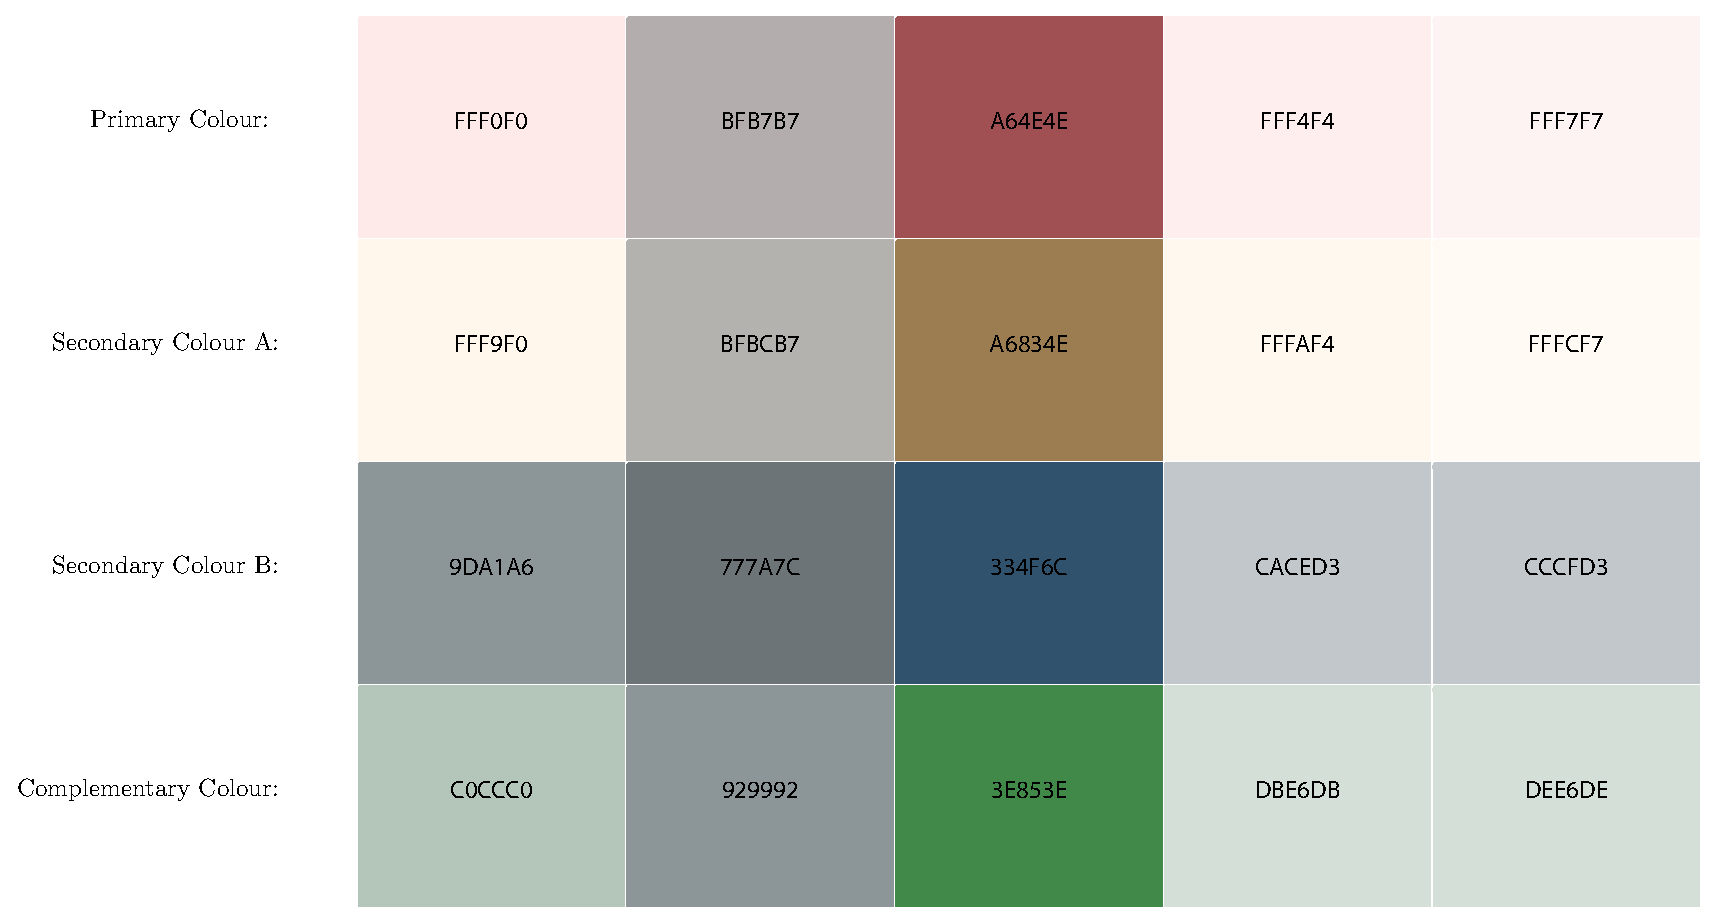
\includegraphics[width=.45\textwidth]{img/colour-scheme}
%	\caption{Colour scheme of the interface \protect\cite{colorschemedesigner.com}}
%	\label{fig:colour-scheme}
%\end{figure}
%\todo[inline]{colorschemedesigner.com cite}
%
%After the navigational structure of the application has been determined
%possible to describe how the system should handle these tasks.
\section{Application Structure}
After the description of the interface, the problem and choice in algorithm it is possible to discuss how the client side should handle user requests and the web server should handle the requests from the client side. In Figure~\ref{fig:use-cases} is shown a use case diagram of how the client side and web server handles use cases.
%\sidecaptionfigure{\textwidth}{img/use-cases}{The figure shows the overall use cases of the system and how the web server acts to accomplish them.}{fig:use-cases}
\begin{figure}[h!tp]
	\myfloatalign
	\makebox[\textwidth][l]{
		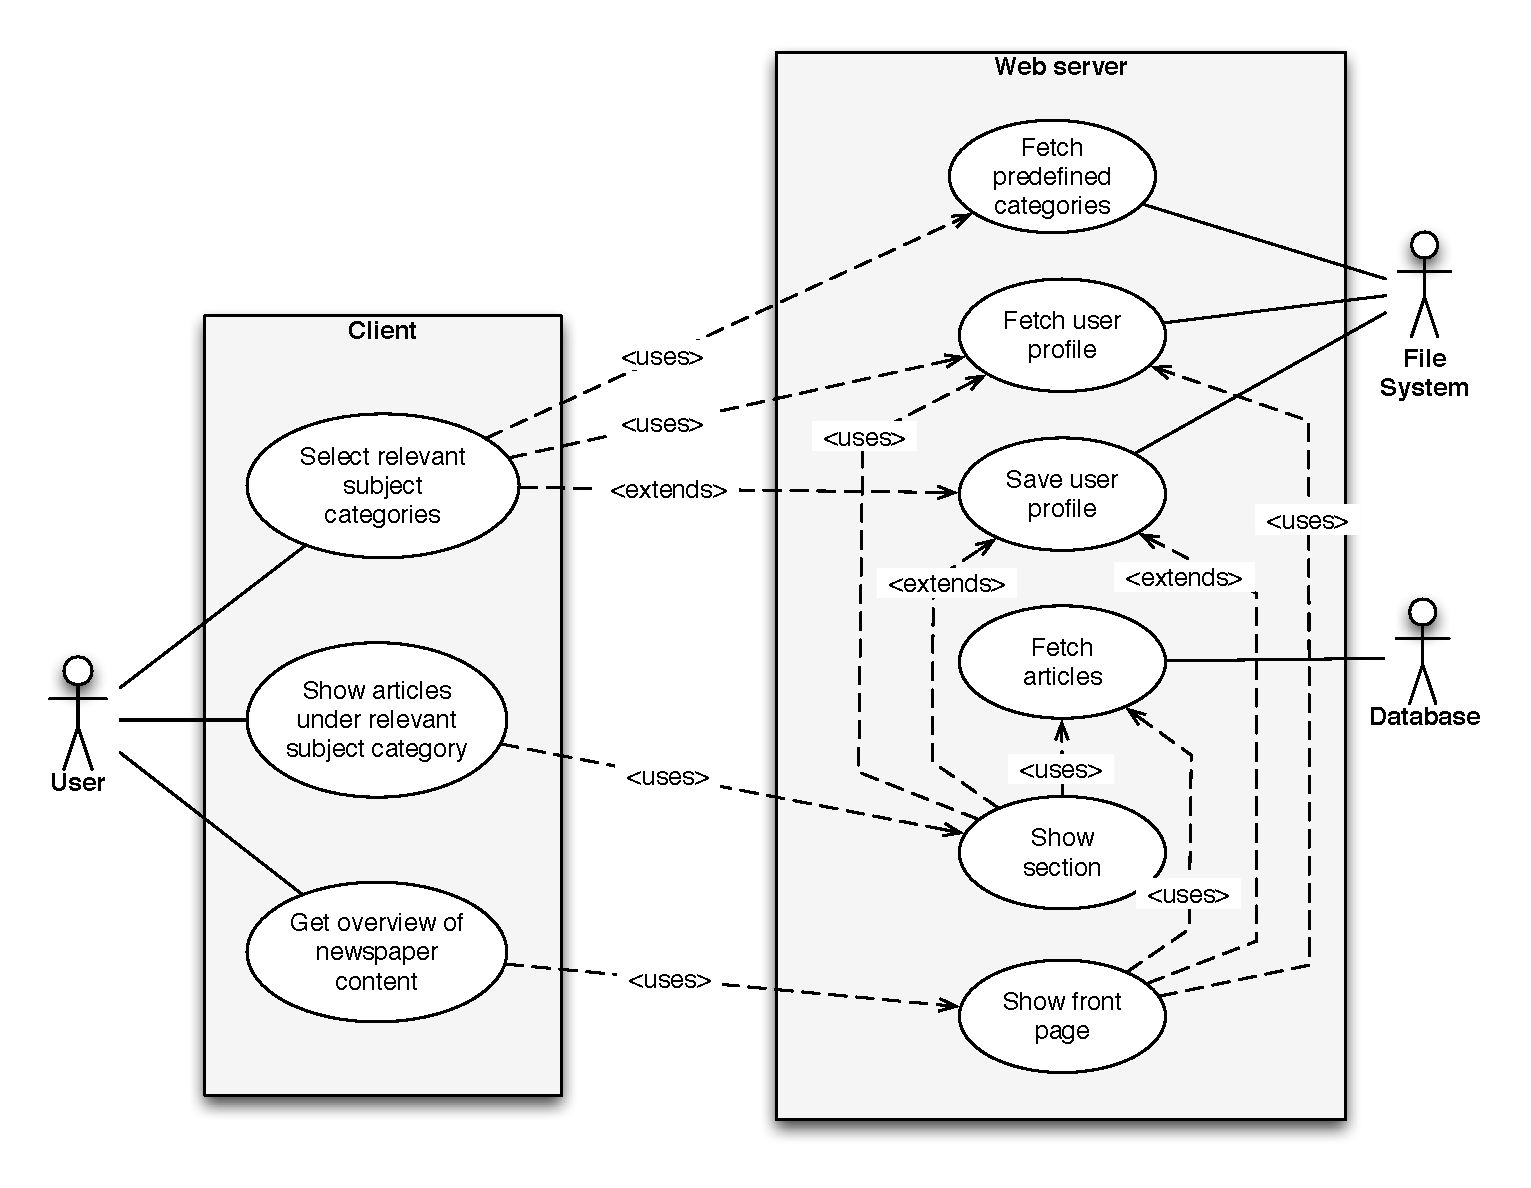
\includegraphics[width=.8\largefigure]{img/use-cases}
	}
	%\marginnote{
		%\begin{minipage}{\marginparwidth}
			\caption{The figure shows the use cases of the system and how the client side handles them and how the web server acts to accomplish requests from the client side.}
			\label{fig:use-cases}
		%\end{minipage}
	%}
\end{figure}

In the diagram and extra use case has been added to show how the system should handle the initial topic selection by the user. The user is able to select relevant topic categories to get an easy start with the application and his choices are thereafter saved to the user profile for later use. The user can thereafter get an overview of the content from the front page or read articles from a selected topic category, both in a nice readable layout and in a composition based on the editorial mix. Moreover, it is possible to an overview of the articles within a section from a the list of headlines from articles contained within it.

The next chapter will present the technical specification of the implementation, which constitutes the product of this project.
%
%\todo[inline]{Which design choices to focus on?}
%

% section design (end)